\section{Performance}

As mentioned previously, the user must specify the requested cluster count \textit{k}. In order to find a suitable value for \textit{k}, the user will need to trial a number of different values. To minimize any negative effect on user-experience, therefore, it is important the clustering performs in near real-time, irrespective of terrain size and cluster count.\\

The performance of the CPU and GPU clustering implementations are analysed below along with an evaluation of the GPU speed-up. In order to evaluate the performance of the different implementations, the clustering time is analysed in relation to terrain size and cluster count. In order to accurately compare their performance, the same terrains are used with identical resources specified. 

\subsection{CPU Performance}

Figure \ref{fig:cpu_clustering_performance} shows the time it takes for the clustering to run with different terrain sizes and number of clusters. Notable results from this data are:
\begin{itemize}
\item Ten clusters take on average five times longer to generate than a single cluster.
\item The same number of clusters take on average four times longer to generate for a terrain of size 512 by 512 than for terrain of size 256 by 256. This increases to six when comparing a terrain of size 512 by 512 with one of size 1024 by 1024.
\end{itemize}

\begin{figure}
\center
	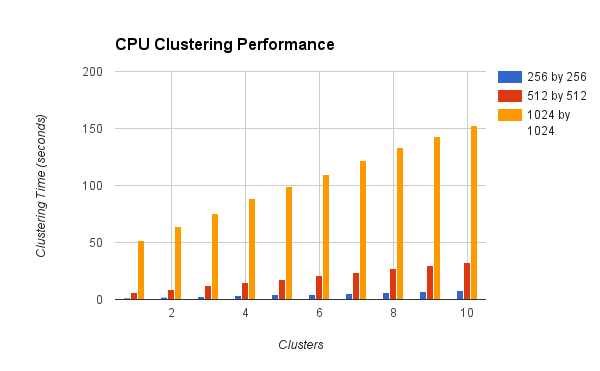
\includegraphics[width=\textwidth]{clustering_cpu_performance.png}
	\caption{ Time it takes for the clustering process to complete on the CPU depending on the cluster count. The analysis was performed for terrains of size: 256 by 256 (blue), 512 by 512 (red) and 1024 by 1024 (orange).}	
	\label{fig:cpu_clustering_performance}
\end{figure}

Although the clustering time is reasonable for smaller terrains, this processing time increases sharply with the terrain size. This is especially true when combined with an increase in the number of clusters to generate. 

\subsection{GPU Performance}

The same tests run using the GPU implementation are displayed in figure \ref{fig:gpu_clustering_performance}. Notable results are:

\begin{itemize}
\item Ten clusters take on average twice the time of a single cluster to generate.
\item The processing time increases proportionally with the number of terrain vertices.
\end{itemize}

\begin{figure}
\center
	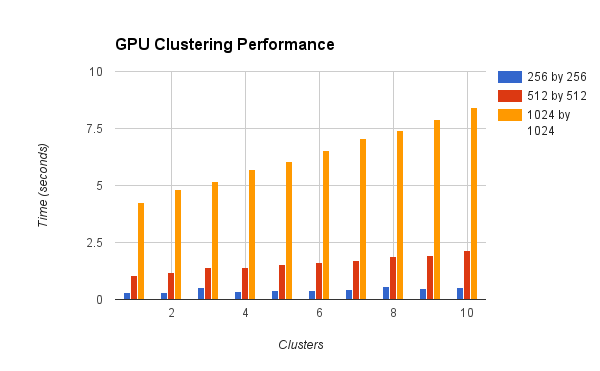
\includegraphics[width=\textwidth]{clustering_gpu_performance.png}
	\caption{ Time it takes for the clustering process to complete on the GPU depending on the cluster count. The analysis was performed for terrains of size: 256 by 256 (blue), 512 by 512 (red) and 1024 by 1024 (orange).}	
	\label{fig:gpu_clustering_performance}
\end{figure}

Because different clusters are managed in parallel on the GPU, increasing the cluster count has a much smaller impact on performance than for the CPU implementation.\\

Individual terrain vertices are managed in parallel on the GPU. Although this greatly speeds up the clustering process, because the number of terrain vertices far outnumber the number of GPU cores, the clustering time is still heavily impacted by increases in terrain size.


\subsection{GPU Speed-up}

Figures \ref{fig:clustering_cpu_v_gpu_256}, \ref{fig:clustering_cpu_v_gpu_512} and \ref{fig:clustering_cpu_v_gpu_1024} compare the CPU and GPU clustering processing time for square terrains of size 256, 512 and 1024 respectively. These graphics show that the GPU greatly outperforms the CPU, irrespective of terrain size and cluster count. Also visible in these graphics is the increased sensitivity to the cluster count of the CPU implementation where the clustering time increases much more rapidly. \\

\begin{figure}
\center
	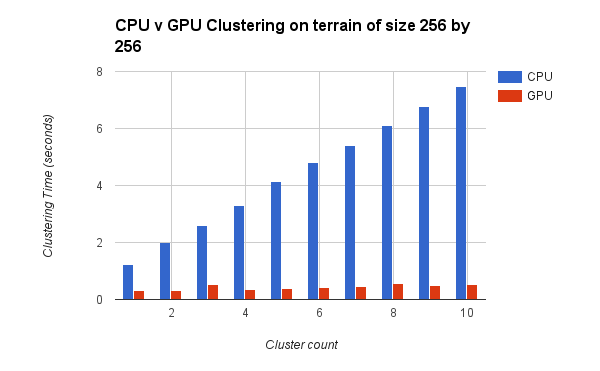
\includegraphics[width=\textwidth]{clustering_cpu_v_gpu_256.png}
	\caption{ Comparison of CPU (blue) and GPU (red) clustering times on a 256 by 256 terrain.}	
	\label{fig:clustering_cpu_v_gpu_256}
\end{figure}

\begin{figure}
\center
	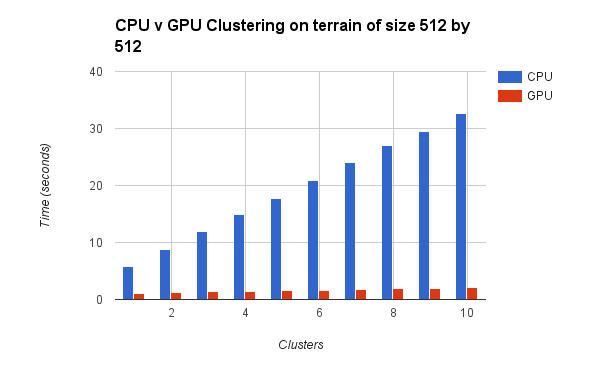
\includegraphics[width=\textwidth]{clustering_cpu_v_gpu_512.png}
	\caption{ Comparison of CPU (blue) and GPU (red) clustering times on a 512 by 512 terrain.}	
	\label{fig:clustering_cpu_v_gpu_512}
\end{figure}

\begin{figure}
\center
	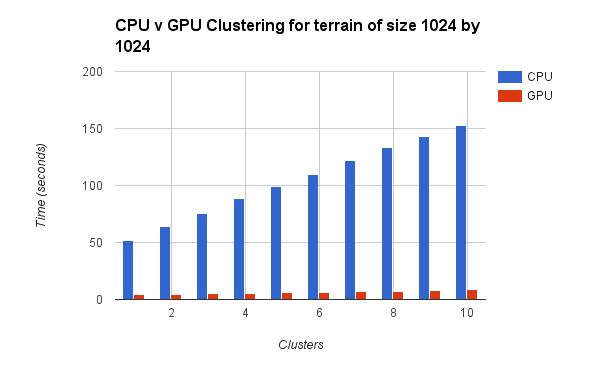
\includegraphics[width=\textwidth]{clustering_cpu_v_gpu_1024.png}
	\caption{ Comparison of CPU (blue) and GPU (red) clustering times on a 1024 by 1024 terrain.}	
	\label{fig:clustering_cpu_v_gpu_1024}
\end{figure}

As well as confirming the increased sensitivity to cluster count of the CPU implementation, figure \ref{fig:clustering_cpu_v_gpu_speedup} which plots the GPU speed-up for each terrain size and cluster count, shows that this speed-up also increases with terrain size. 

\begin{figure}
\center
	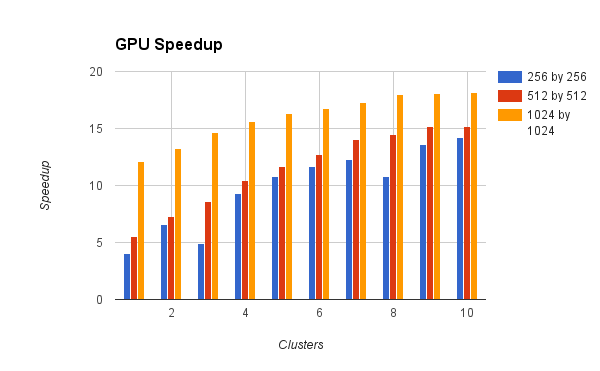
\includegraphics[width=\textwidth]{clustering_cpu_v_gpu_speedup.png}
	\caption{ Calculated clustering speed-up of the GPU implementation compared to the CPU implementation for square terrains of size 256 (blue), 512 (red) and 1024 (yellow).}	
	\label{fig:clustering_cpu_v_gpu_speedup}
\end{figure}